\documentclass[10pt,landscape]{article}
\usepackage{multicol}
\usepackage{calc}
\usepackage{ifthen}
\usepackage[landscape]{geometry}
\usepackage{hyperref}
\usepackage{graphicx}
\usepackage{amsmath,amssymb}
\usepackage{algorithm2e}
\usepackage{subcaption}
\usepackage{float}

% To make this come out properly in landscape mode, do one of the following
% 1.
%  pdflatex rl_cheatsheet.tex
%
% 2.
%  latex rl_cheatsheet.tex
%  dvips -P pdf  -t landscape rl_cheatsheet.dvi
%  ps2pdf rl_cheatsheet.ps


% If you're reading this, be prepared for confusion.  Making this was
% a learning experience for me, and it shows.  Much of the placement
% was hacked in; if you make it better, let me know...


% 2008-04
% Changed page margin code to use the geometry package. Also added code for
% conditional page margins, depending on paper size. Thanks to Uwe Ziegenhagen
% for the suggestions.

% 2006-08
% Made changes based on suggestions from Gene Cooperman. <gene at ccs.neu.edu>


% To Do:
% \listoffigures \listoftables
% \setcounter{secnumdepth}{0}


% This sets page margins to .5 inch if using letter paper, and to 1cm
% if using A4 paper. (This probably isn't strictly necessary.)
% If using another size paper, use default 1cm margins.
\ifthenelse{\lengthtest { \paperwidth = 11in}}
        { \geometry{top=.5in,left=.5in,right=.5in,bottom=.5in} }
        {\ifthenelse{ \lengthtest{ \paperwidth = 297mm}}
                {\geometry{top=1cm,left=1cm,right=1cm,bottom=1cm} }
                {\geometry{top=1cm,left=1cm,right=1cm,bottom=1cm} }
        }

% Turn off header and footer
\pagestyle{empty}


% Redefine section commands to use less space
\makeatletter
\renewcommand{\section}{\@startsection{section}{1}{0mm}%
                                {-1ex plus -.5ex minus -.2ex}%
                                {0.5ex plus .2ex}%x
                                {\normalfont\large\bfseries}}
\renewcommand{\subsection}{\@startsection{subsection}{2}{0mm}%
                                {-1explus -.5ex minus -.2ex}%
                                {0.5ex plus .2ex}%
                                {\normalfont\normalsize\bfseries}}
\renewcommand{\subsubsection}{\@startsection{subsubsection}{3}{0mm}%
                                {-1ex plus -.5ex minus -.2ex}%
                                {1ex plus .2ex}%
                                {\normalfont\small\bfseries}}

\newcommand\numberthis{\addtocounter{equation}{1}\tag{\theequation}}

\makeatother

% Define BibTeX command
\def\BibTeX{{\rm B\kern-.05em{\sc i\kern-.025em b}\kern-.08em
    T\kern-.1667em\lower.7ex\hbox{E}\kern-.125emX}}

% Don't print section numbers
\setcounter{secnumdepth}{0}


\setlength{\parindent}{0pt}
\setlength{\parskip}{0pt plus 0.5ex}

\DeclareMathOperator*{\argmax}{argmax}

% -----------------------------------------------------------------------

\begin{document}

\raggedright
\footnotesize
\begin{multicols}{3}

% multicol parameters
% These lengths are set only within the two main columns
%\setlength{\columnseprule}{0.25pt}
\setlength{\premulticols}{1pt}
\setlength{\postmulticols}{0.1pt}
\setlength{\multicolsep}{1pt}
\setlength{\columnsep}{1pt}

\begin{center}
     \Large{Reinforcement Learning Cheat Sheet} \\
\end{center}
\subsection{Recap}
$\mathbb{E}[X] \stackrel{.}{=} \sum_{x_i} x_i \cdot Pr\{ X = x_i \}$
$\mathbb{E}[X | Y = y_j] = \sum_{x_i} x_i \cdot Pr\{ X = x_i | Y = y_j\}$
$\mathbb{E}[X | Y = y_j] = \sum_{z_k} Pr\{Z=z_k | Y = y_j\} \cdot \mathbb{E}[X|Y = y_j, Z = z_k]$

\subsection{Agent-Environment Interface}
\begin{center}
\includegraphics[width=\linewidth]{./images/Agent-Environment.png}
\end{center}
The Agent at each step $t$ receives a representation of the environment's \emph{state} $S_t \in \mathcal{S}$ and it selects an action $A_t \in \mathcal{A}(s)$. One time step later, as a consequence of its action, the agent receives a \emph{reward}, $R_{t + 1} \in \mathcal{R} \subseteq \mathbb{R}$ and goes to the new state $S_{t+1}$.

\subsection{Multi-Armed Bandits}

\subsection{Markov Decision Process (MDPs)}
\textbf{Backup Diagrams} diagram the relationships that form the basis of \textit{backup} operations which transfer value information back to a state (or state-action pair) form its successor states (or state-action pairs). \\

A finite \textbf{Markov Decision Process}, MDP, is defined by:
\begin{enumerate}
    \item finite set of states:  $s \in \mathcal{S}$,
    \item finite set of actions: $a \in \mathcal{A}$
    \item dynamics:
\begin{equation}
p(s', r | s, a) \stackrel{.}{=} Pr \{S_{t} = s', R_{t} = r | \\ S_{t-1} = s, A_{t-1} = a \} \quad [3.2] \numberthis
\end{equation}
    \item state transition probabilities: 
\begin{align*}
p(s' | s, a) & \stackrel{.}{=} Pr \{S_{t} = s' | S_{t-1} = s, A_{t-1} = a \} \\
& = \sum_{r \in \mathcal{R}} p(s', r | s, a) \quad [3.4]  \numberthis
\end{align*}
    \item expected reward for state-action:
\begin{align*}
r(s, a) & \stackrel{.}{=} \mathbb{E}[ R_{t} | S_{t-1} = s, A_{t-1} = a ] \\
 & = \sum_{r \in \mathcal{R}} r \cdot \sum_{s' \in \mathcal{S}} p(s', r | s, a) \quad [3.5]  \numberthis
\end{align*}
    \item expected reward for state-action-next state: 
\begin{align*}
r(s',s, a) & \stackrel{.}{=} \mathbb{E}[ R_{t} | S_{t-1} = s, A_{t-1} = a, S_{t} = s' ] \\
& = \sum_{r \in \mathcal{R}} r \cdot \frac{p(s', r | s, a)}{p(s' | s,a)} \quad [3.6] \numberthis
\end{align*}
\end{enumerate}

The MDP and agent together thereby give rise to a sequence or \emph{trajectory} that begins like this:
$S_0,A_0,R_1,S_1,A_1,R_2,S_2,A_2,R_3...$

\subsection{Return}
In RL the goal of the agent is not the maximization of the immediate reward, but of the cumulative reward in the long run. The \emph{return} is a specific function of reward sequence. In the simplest case the return is the sum of rewards: 
\begin{equation}
G_t \stackrel{.}{=} R_{t+1} + R_{t+2} + R_{t+3} + ... +  R_{T} \numberthis \label{eq:return_1} \quad [3.7]
\end{equation}
where $T$ is a final time step. \\

When there is a natural notion of final time step ($T$), the agent-environment interaction breaks naturally into sub-sequences (\emph{episodes}) and the next episode begins independently of how the previous one ended. Tasks with episodes are called \emph{episodic tasks}. \\

Each episodes ends in a special state called \emph{terminal state} with different rewards for the different outcomes.  $\mathcal{S}^{+}$ is the set of all states plus the terminal state.

When the agent-environment interaction does not break naturally into episodes but goes on continually without limit, we call these \emph{continuing tasks}.
The previous formulation of return (Eq. \ref{eq:return_1}) is problematic because $T=\infty$. 

The \emph{total discounted return} expressed as the sum of rewards (opportunely discounted using the \emph{discount rate} $0 \le \gamma \le 1$):
\begin{align*}
G_t & \stackrel{.}{=} R_{t+1} + \gamma R_{t+2} + \gamma^2 R_{t+3} + ...\\
& = \sum_{k = 0}^\infty \gamma^k R_{t + k + 1} \numberthis \label{eq:discounted_return_1} \quad [3.8]\\
& = R_{t+1} + \gamma G_{t+1} \numberthis \label{eq:discounted_return_2} \quad [3.9]
\end{align*}

To unify the notation for episodic and continuing tasks we use:

\begin{equation}
G_t \stackrel{.}{=} \sum_{k = t+1}^T \gamma^{k-t-1} R_{k} \numberthis \label{eq:discounted_return_generic} \quad [3.11]
\end{equation}

including the possibility that $T=\infty$ or $\gamma = 1$ \emph{but not both}.
\subsection{Policy}
A \emph{policy} is a mapping from a state to probabilities of selecting each possible action:
\begin{equation}
\pi(a|s)
\label{eq: policy}
\end{equation}
That is the probability of select an action $A_t = a$ if $S_t = s$.

\subsection{Value Functions}
\emph{State-Value function} describes \emph{how good} it is to be in a specific state $s$ under a certain policy $\pi$.
It is the expected return (expected cumulative discounted reward) when starting from $s$ and following $\pi$. For any policy $\pi$ and $\forall s \in \mathcal{S}$:
\begin{align*}
v_{\pi}(s) & \stackrel{.}{=} \mathbb{E}_{\pi}[G_t | S_t = s] \numberthis \label{eq:v_def} \quad [3.12] \\
& = \mathbb{E}_{\pi}[R_{t+1} + \gamma G_{t+1} | S_t = s] \numberthis  \quad [by \ 3.9] \\
& = \sum_{a} \pi(a|s) \sum_{s' ,r} p(s',r | s, a) \Big[r + \gamma v_{\pi}(s')\Big] \numberthis \label{eq:v_bellman} \quad [3.14]
\end{align*}
The last one is the \textbf{Bellman equation for $v_\pi$}.

\emph{Action-Value function (Q-Function)} describes \emph{how good} is to perform a given action $a$ in a given state $s$ under a certain policy $\pi$. It is the expected return when starting from $s$, taking action $a$ and thereafter following $\pi$:
\begin{align*}
q_{\pi}(s,a) & \stackrel{.}{=} \mathbb{E}_{\pi}[G_t | S_t = s, A_t = a]  \numberthis \label{eq:q_def}\quad [3.13] \\
& = \sum_{s',r} p(s',r|s,a) \Big[r + \gamma \sum_{a'} \pi(a'|s') q_{\pi}(a',s') \Big]  \numberthis \label{eq:q_bellman}\quad [Ex \ 3.17]
\end{align*}
The last one is the \textbf{Bellman equation for $q_\pi$}.
\vfill\null

\subsubsection{Relation between Value Functions}
\begin{align*}
v_{\pi}(s) & = \sum_{a} \pi(a|s) \cdot q_{\pi}(s,a)  \numberthis \label{eq:v_derived_1} \quad [Ex \ 3.12] \\
& = \mathbb{E}_{\pi}[ q_{\pi}(s,a) | S_t = s] \numberthis \label{eq:v_derived_2} \quad [Ex \ 3.18]
\end{align*}
\begin{align*}
q_{\pi}(s,a) & =  \sum_{s',r} p(s',r|s,a) \Big[r + \gamma v_{\pi}(s')\Big] \numberthis \label{eq:q_derived_1} \quad [Ex \ 3.13]\\
& = \mathbb{E} \Big[ R_{t+1} + \gamma v_{\pi}(s') | S_t = s, A_t = a \Big]  \numberthis \label{eq:q_derived_2} \quad [Ex \ 3.19]
\end{align*}

\begin{center}
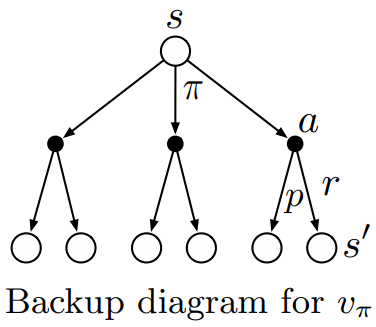
\includegraphics[width=0.45\linewidth]{./images/v_backup.png}
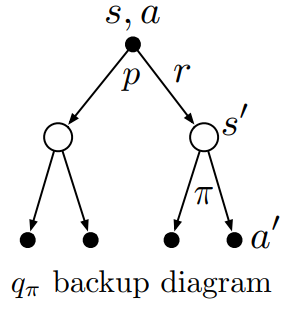
\includegraphics[width=0.45\linewidth]{images/q_backup.png}
\end{center}

\subsection{Optimal Value Functions}
\begin{align*}
v_*(s) & \stackrel{.}{=} \max\limits_{\pi} v_\pi(s) \numberthis  \label{eq: value_optimal} \quad [3.15]\\
& = \max_a \mathbb{E} [R_{t+1} + \gamma v_{*}(S_{t+1}) | S_{t} = s, A_t = a ] \quad [3.18]\\
& = \max_a \sum_{s',r} p(s',r|s,a) \Big[r + \gamma v_{*}(s') \Big] \quad [3.19]
\end{align*}

\begin{align*}
q_*(s,a) & \stackrel{.}{=} \max\limits_{\pi} q_\pi(s,a) \numberthis  \label{eq: action_value_optimal} \quad [3.16]\\
& = \mathbb{E} [R_{t+1} + \gamma \max_{a'} q_{*}(S_{t+1}, a') | S_{t} = s, A_t = a ] \\
& = \sum_{s',r} p(s',r|s,a) \Big[r + \gamma \max_{a'} q_{*}(s',a')\Big] \quad [3.20] 
\end{align*}

\begin{equation}
v_*(s) = \max\limits_{a \in A(s)} q_{\pi_*}(s,a)
\end{equation}
Intuitively, the above equation express the fact that the value of a state under the optimal policy \textbf{must be equal} to the expected return from the best action from that state.

\subsubsection{Relation between Optimal Value Functions}
\begin{align*}
v_{*}(s) & = \max_a \sum_{s',r} p(s',r|s,a) \Big[r + \gamma \sum_{a'} \pi(a'|s') q_{*}(s',a')\Big] \quad [Ex \ 3.25] \numberthis \label{eq:vstar_derived_1}\\
\end{align*}
\begin{align*}
q_{*}(s,a) & = \sum_{s',r} p(s',r|s,a) \Big[r + \gamma v_{*}(s') \Big]  \quad [Ex \ 3.26] \numberthis \label{eq:qstar_derived_1}\\
\end{align*}
% \end{multicols}

\begin{center}
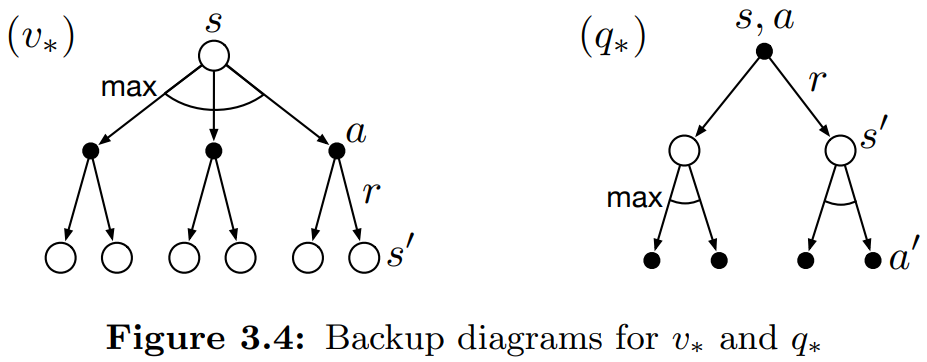
\includegraphics[width=\linewidth]{images/optimal_backup.png}
\end{center}


% \newpage

% \begin{multicols}{3}

\section{Dynamic Programming}
Collection of algorithms that can be used to compute optimal policies given a perfect model of the environment as a MDP. 

\textbf{Prediction} estimating the value of states or state-action pairs given a fixed policy. \\
\textbf{Control} Finding an optimal policy that maximises over cumulative rewards.

\subsection{Policy Evaluation [Prediction]}
If the environment's dynamic is completely known, the Eq. \ref{eq:v_bellman} is a system of $|\mathcal{S}|$ equations in  $|\mathcal{S}|$ unknowns ($v_\pi(s), s \in \mathcal{S}$). \\
We also can use an iterative solution,  $\forall s \in \mathcal{S}$:
\begin{align*}
v_{k+1}(s) & \stackrel{.}{=} \mathbb{E}_{\pi}[R_{t+1} + \gamma v_{k}(S_{t+1}) | S_t = s] \\
& = \sum_{a} \pi(a|s) \sum_{s' ,r} p(s',r | s, a)  [r + \gamma v_{k}(s')] \numberthis  \quad [4.5]
\end{align*}
We can compute new values $v_{k+1}(s)$ from old values $v_k(s)$ without change old values or update the values \emph{in-place}.

% \subsubsection{Iterative Policy Evaluation for estimating $V \sim v_{\pi}$ (in-place version)}
% \begin{algorithm}[H]
% Inputs: $\pi$ - the policy to be evaluated \\
% Params: $\theta$ - a small positive threshold determining the accuracy of the estimation \\
% Initialize V(s), for all $s \in \mathcal{S}^{+}$ arbitrarily, except V(terminal) = 0\\
%  $\Delta \leftarrow 0$ \\
%  \While{$\Delta \ge \theta$}
%  {
%   \ForEach{$s \in S$} {
%         $v \leftarrow V(s)$\\
%         $V(s) \leftarrow \sum\limits_a \pi(a|s) \sum\limits_{s', r} p(s',r | s, a) \begin{bmatrix}
%                 r + \gamma V(s')
%         \end{bmatrix}$ \\
%         $\Delta \leftarrow \max(\Delta, | v - V(s)|)$
%         }
% }
% \caption{Iterative Policy Evaluation - estimating $V \sim v_{\pi}$ - [§4.1]}
% \end{algorithm}

% The algorithm tests the quantity $\max_{s \in \mathcal{S}} |v_{k+1}(s) - v_k(s)|$ after each \emph{sweep} and stops when it is sufficiently small ($\Delta < \theta$).
%\vfill\null
%\columnbreak

\subsection{Policy Iteration}
Policy iteration consists of two simultaneous, interacting processes: one making the value function consistent with the current policy (\emph{policy evaluation}), and the other making the policy greedy with respect to the current value function (\emph{policy improvement}). 
\begin{algorithm}[H]
%\SetAlgoLined
 1. Initialization \\
 Assign arbitrarily $V(s) \in \mathbb{R}$ and $\pi(s) \in \mathcal{A}(s)$  for all $s \in S$,\\
 2. Policy Evaluation \\
 $\Delta \leftarrow 0$ \\
 \While{$\Delta \ge \theta$}
 {
  \ForEach{$s \in S$} {
        $v \leftarrow V(s)$\\
        $V(s) \leftarrow \sum\limits_a \pi(a|s) \sum\limits_{s', r} p(s',r | s, a) \begin{bmatrix}
                r + \gamma V(s')
        \end{bmatrix}$ \\
        $\Delta \leftarrow \max(\Delta, | v - V(s)|)$
        }
}
 3. Policy Improvement \\
 \emph{policy-stable} $ \leftarrow $ \emph{true} \\
  \ForEach{$s \in S$} {
        \emph{old-action} $\leftarrow \pi(s)$\\
        $\pi(s) \leftarrow \argmax\limits_a\sum\limits_{s', r} p(s',r | s, a)  \begin{bmatrix}
            r + \gamma V(s')
        \end{bmatrix}$ \\
        \If{\emph{old-action} $\neq \pi(s)$}
        {
        	\emph{policy-stable} $\leftarrow$ \emph{false}
        }
  }
\uIf{\emph{policy-stable}}
{
	return V $\approx v_*$ and $\pi \approx \pi_*$
}
\Else
{
	go to 2
}

\caption{Policy Iteration - estimating $\pi \sim \pi_*$ - deterministic policy - [§4.3]}
\end{algorithm}

\subsection{Value Iteration}
Instead of waiting the convergence of $V(s)$ (policy evaluation loop) we can perform only one step of policy evaluation that, combined with policy improvement, lead to the following formulation:
\begin{align*}
v_{k+1}(s) & = \max_a \mathbb{E}_{\pi}[R_{t+1} + \gamma v_{k}(S_{t+1}) | S_t = s] \\
& = \max_a \sum_{s' ,r} p(s',r | s, a)  [r + \gamma v_{k}(s')] \numberthis  \quad [4.10]
\end{align*}

\begin{algorithm}[H]
Params: $\theta$ - a small positive threshold determining the accuracy of the estimation \\
Initialize V(s), for all $s \in \mathcal{S}^{+}$ arbitrarily, except V(terminal) = 0\\
\SetKwInOut{Output}{output}
 $\Delta \leftarrow 0$ \\
\While{$\Delta \ge \theta$}
{
  \ForEach{$s \in S$} {
        $v \leftarrow V(s)$\\
        $V(s) \leftarrow \max\limits_a \sum\limits_{s', r} p(s',r | s, a) \begin{bmatrix}
                r + \gamma V(s')
        \end{bmatrix}$ \\
        $\Delta \leftarrow \max(\Delta, | v - V(s)|)$
        }
}

 \Output{Deterministic policy $\pi \approx \pi_*$ such that}
 $\pi(s) = \argmax\limits_a \sum\limits_{s', r} p(s',r | s, a) \begin{bmatrix}
     r + \gamma V(s')
  \end{bmatrix}$
\caption{Value Iteration - estimating  $\pi \sim \pi_*$ - [§4.4]}
\end{algorithm}
One \emph{sweep} is one update of each state.\\
In value iteration only a single iteration of policy evaluation is performed between each policy improvement. 
Value iteration combines, in each of its sweeps, one sweep of policy evaluation and one sweep of policy improvement.\\ Faster convergence is often achieved by interposing multiple policy evaluation sweeps between each policy improvement sweep.

\subsection{Generalized Policy Iteration}
Generalized Policy Iteration is a way to refer to the general idea of letting policy-evaluation and policy-improvement processes interact, independent of the granularity and other details of the two processes. \\
Almost all reinforcement learning methods are well described as GPI. That is, all have identifiable policies and value functions, with the policy always being improved with respect to the value function and the value function always being driven toward the value function for the policy, as suggested by the diagram below [§4.6]:
\begin{center}
\includegraphics[width=0.5\linewidth]{./images/GPI.png}
\end{center}

% \end{multicols}

% \newpage

% \begin{multicols}{3}

\section{Monte Carlo Methods}
Monte Carlo (MC) methods require only experience from actual or simulated environment.

\subsection{MC Prediction}
\begin{algorithm}[H]
Inputs: $\pi$ - the policy to be evaluated \\
Initialize: $V(s) \in \mathbb{R}$ for all $s \in \mathcal{S}$ \\
$\text{Return(s)} \leftarrow \text{an empty list}$ for all $s \in \mathcal{S}$ \\
\While{forever - for each episode}
{
    Generate an episode following $\pi$: $S_0, A_0, R_1, S_1, A_1,..., S_{T-1}, A_{T-1}, R_T$\\
    $G \leftarrow$ 0 \\
    \ForEach{step of episode, $t=T-1, T-2, ..., 0$}
    {
    	$G \leftarrow \gamma G + R_{t+1}$\\
       \If{$S_t$ is not in the sequence $S_0, S_1,..., S_{t-1}$ (i.e. it is the first visit to $S_t$) }
        {
        	Append $G$ to Return($S_t$)\\
        	$V(S_t) \leftarrow$ average(Return($S_t$))
        }
    }
 }
\caption{On-policy First-visit Monte Carlo prediction - estimating $V \sim v_{\pi}$ [§5.1]}
\end{algorithm}
The \emph{first-visit} is the first time a particular state has been observed.\\		
The \textbf{first-visit MC} method estimates $v_{\pi}(s)$ as the average of the returns following first visits to $s$, whereas the \textbf{every-visit MC} method averages the returns following all visits to $s$.
The every-visit MC Prediction is derived from first-visit version removing the ``if'' condition. \\
In other words we move backward from the step $T$ and compute the $G$ incrementally and associate the values of $G$ to the current state and perform the average.

\subsection{MC Estimation of Action Values}
To determine a policy, if a model is not available, the state value is not sufficient and we have to estimate the values of state–action pairs. \\


The only complication is that many state–action pairs may never be visited.  We need to estimate the value of all the actions from each state, not just the one we currently favor. 
We can specify that the episodes start in a state–action pair, and that every pair has a nonzero probability of being selected as the start (assumption of \emph{exploring starts}). \\

\subsection{MC Control}
\begin{algorithm}[H]
 Initialise:
	$\pi(s) \in \mathcal{A}(s)$ arbitrarily, for all $s \in \mathcal{S}$ \\       
       $Q(s,a) \in \mathbb{R}$ (arbitrarily) for all $s \in \mathcal{S}, a \in \mathcal{A}(s)$ \\
       $ Returns(s,a) \leftarrow \text{empty list}$ for all $s \in \mathcal{S}, a \in \mathcal{A}(s)$ \\

 \While{forever}{
    Choose $S_0 \in S$ and $A_0 \in A(S_0)$, randomly such that all pairs have probability $ > 0$ \\
    Generate an episode from $S_0, A_0$ following $\pi: S_0, A_0, R_1,...,S_{T-1},A_{T-1},R_T$\\
    $G \leftarrow 0$ \\
    \ForEach{step of episode, $t=T-1, T-2, ..., 0$}
    {
    	$G \leftarrow \gamma G + R_{t+1}$\\
       \If{$S_t, A_t$ pair is not seen before, is not in the sequence $S_0, A_0, S_1, A_1..., S_{t-1}, A_{t-1}$ }
        {
        	Append $G$ to Returns($S_t, A_t$)\\
        	$Q(S_t, A_t) \leftarrow$ average(Returns($S_t,A_t$))\\
        	$\pi(S_t) \leftarrow \argmax_a (Q(S_t, a))$
        }
    }
 }
\caption{First-visit Monte Carlo (Exploring Starts) - estimating $\pi \sim \pi_*$ [§5.3]}
\end{algorithm}

To remove the exploring starts assumption, we can use an $\epsilon-$soft policy. Most of times it selects the greedy policy but with probability $\epsilon$ it instead selects an action at random. \\

Other approaches are the \emph{off-policy} methods that learn about the optimal policy while behaving according to a different exploratory policy.
The policy being learned about is called the \emph{target policy}, $\pi$, and the policy used to generate behaviour is called the \emph{behaviour policy}, $b$ (usually an exploratory policy, e.g. random policy). \\

\textbf{Assumption of Coverage} In order to use episodes from $b$ to estimate values for $\pi$, we require that every action taken under $\pi$ is also taken, at least occasionally, under $b$. That is, we require that $\pi(a|s) > 0$ implies $b(a|s) > 0$.

\subsection{Off-policy Every-visit MC Prediction}
\begin{algorithm}[H]
Inputs: $\pi$ - the policy to be evaluated \\
Initialize: $V(s) \in \mathbb{R}$ for all $s \in \mathcal{S}$ \\
$\text{Return(s)} \leftarrow \text{an empty list}$ for all $s \in \mathcal{S}$ \\
\While{forever - for each episode}
{
    Generate an episode following $b$: $S_0, A_0, R_1, S_1, A_1,..., S_{T-1}, A_{T-1}, R_T$\\
    $G \leftarrow$ 0 \\
    $W \leftarrow$ 1 \\
    \ForEach{step of episode, $t=T-1, T-2, ..., 0$}
    {
    	$G \leftarrow \gamma W G + R_{t+1}$\\
	Append $G$ to Return($S_t$)\\
	$V(S_t) \leftarrow$ average(Return($S_t$))
	$W \leftarrow W \frac{\pi(A_t|S_t)}{b(A_t|S_t)}$
    }
 }
\caption{Off-policy Every-visit Monte Carlo prediction - estimating $V \sim v_{\pi}$}
\end{algorithm}

\subsubsection{Importance Sampling Ratio}

\subsection{Incremental Implementation}
The average used to compute $V(S_t)$, can be performed incrementally:
\begin{align*}
V_n(S_t) = \frac{1}{n} \sum_{i=1}^{n} G_i(t) = V_{n-1}(S_t) + \frac{1}{n} (G_n(t) - V_{n-1}(S_t)) \label{eq:incremental_mc}\numberthis
\end{align*}

\subsection{Off-policy MC Control}
An advantage of the separation of the target and behaviour policy is that the target policy may be deterministic (e.g., greedy), while the behaviour policy can continue to sample all possible actions.
\begin{algorithm}[H]
Initialize:for all $s \in \mathcal{S}$, $a \in \mathcal{A}(s)$ \\
	$Q(s, a) \in \mathbb{R}$ 
 	$C(s,a) \leftarrow 0$
 	$\pi(s) \leftarrow \argmax_a +Q(s,a)$

\While{forever - for each episode}
{
	$b \leftarrow \text{any soft policy}$
    	Generate an episode following $b$: $S_0, A_0, R_1, S_1, A_1,..., S_{T-1}, A_{T-1}, R_T$\\
    	$G \leftarrow$ 0 \\
    	$W \leftarrow$ 1 \\
    	\ForEach{step of episode, $t=T-1, T-2, ..., 0$}
    	{
    		$G \leftarrow \gamma G + R_{t+1}$ \\
    		$C(S_t,A_t) \leftarrow C(S_t,A_t) + W$ \\
    		$Q(S_t,A_t) \leftarrow Q(S_t,A_t) + \frac{W}{C(S_t,A_t)}[G - Q(S_t,A_t)]$ \\
    		$\pi(s) \leftarrow \argmax_a +Q(S_T,a)$ \\
		\If{$A_t \neq \pi(S_t)$}
        	{
        		exit For Loop
		}
		$W \leftarrow W \frac{1}{b(A_t|S_t)}$
    }
 }
\caption{Off-policy MC Control - estimating $\pi \sim \pi_*$ [§5.7]}
\end{algorithm}

% \end{multicols}

% \newpage

% \begin{multicols}{3}

\section{Temporal-Difference Learning}

\subsection{TD Prediction}
Starting from Eq. \ref{eq:incremental_mc}, we can consider a generic update rule of $V(S_t)$

\begin{align*}
V(S_t) \leftarrow V(S_t) + \alpha (\mathbf{G_t} - V(S_t)) \label{eq:constant_alpha_mc}\numberthis \quad [6.1]
\end{align*}
$\alpha$ is a constant step-size and we call previous method \emph{constant-$\alpha$ MC}.
MC has to wait the end of an episode to determine the increment to $V(S_t)$. \\
Differently from MC, TD updates the value at each step of the episode following the equation below:

\begin{align*}
V(S_t) \leftarrow V(S_t) + \alpha (\mathbf{R_{t+1} + \gamma V(S_{t+1})} - V(S_t)) \label{eq:td_0}\numberthis \quad [6.2]
\end{align*}

\begin{algorithm}[H]
Inputs: $\pi$ - the policy to be evaluated \\
Params: step size $\alpha \in [0,1]$ \\
Initialize: $V(s) \in \mathbb{R}$ for all $s \in \mathcal{S}^+$ except for V(terminal)=0 \\

\ForEach{episode}
{
    Initialize $S$\\
    \ForEach{step of episode - until $S$ is terminal}
    {
    	$A \leftarrow$ action given by $\pi$ for S\\
    	Take action $A$, observe $R$, $S'$\\
    	$V(S) \leftarrow V(S) + \alpha (R + \gamma V(S') - V(S))$ \\
    	$S \leftarrow S'$   
    }
 }
\caption{Tabular TD(0) - estimating $v_{\pi}$ [§6.1]}
\end{algorithm}

Recall that:
\begin{align*}
v_{\pi}(s) & \stackrel{.}{=} \mathbb{E}_{\pi}[G_t | S_t = s]  \label{eq:v_pi_MC} \numberthis  \quad [3.12 | 6.3]\\
& = \mathbb{E}_{\pi}[R_{t+1} + \gamma G_{t+1} | S_t = s] \label{eq:v_pi_MC2}  \numberthis  \quad [by \ 3.9] \\
& = \mathbb{E}_{\pi}[R_{t+1} + \gamma v_{\pi}(S_{t+1}) | S_t = s] \label{eq:v_pi_TD} \numberthis  \quad [6.4] \\
\end{align*}
MC methods use an estimate of Eq. \ref{eq:v_pi_MC} as a target. 
The MC target is an estimate because the expected value in Eq. \ref{eq:v_pi_MC} is not known; a sample return is used in place of the real expected return.\\

DP and TD methods use an estimate of Eq. \ref{eq:v_pi_TD} as a target.\\
The DP target is an estimate because $v_{\pi}(S_{t+1})$ is not known and the current estimate, $V(S_{t+1})$, is used instead. \\
The TD target is an estimate because it samples the expected values in Eq. \ref{eq:v_pi_TD} and it uses the current estimate $V$ instead of the true $v_{\pi}$.\\

TD methods update their estimates based in part on other estimates. They learn a guess from a guess, i.e. they \textbf{bootstrap}.
TD and MC methods have an advantage over DP methods in that they do not require a model of the environment, of its reward and next-state probability distributions.

The most obvious advantage of TD methods over MC methods is that they are naturally implemented in an online, fully incremental fashion. 
With MC methods one must wait until the end of an episode, because only then the return is known, whereas with TD methods one needs wait only one time step.
In practice, TD methods have usually been found to converge faster than constant-$\alpha$ MC methods on stochastic tasks.\\
The error, available at time $t+1$, between $V(S_t)$ and the better estimate $R_{t+1} + \gamma V(S_{t+1})$ is called \emph{TD error}:
\begin{equation*}
\delta_t \stackrel{.}{=} R_{t+1} + \gamma V(S_{t+1}) - V(S_t) \numberthis  \quad [6.5]
\end{equation*}

\subsection{Sarsa - On-policy TD Control}
Sarsa (State-action-reward-state-action) is an on-policy TD control. 
Sarsa is sample-based version of policy iteration which uses Bellman equations for action values. 
The update rule:

\begin{align*}
    Q(S_t, A_t) \leftarrow & \\
    Q(S_t, A_t) + & \alpha \left[R_{t+1} + \gamma Q(S_{t+1}, A_{t+1}) - Q(S_t, A_t) \right] \numberthis  \quad [6.7]
\end{align*}

\begin{algorithm}[H]
 Params: step size $\alpha \in [0,1]$, $\epsilon > 0$ \\
 Initialize $Q(s,a)$ for all $s \in \mathcal{S}^+$ and $a \in \mathcal{A}(s)$, arbitrarily except that $Q(terminal-state, \cdot) = 0$\\
\ForEach{episode}
{
    Initialize $S$\\
    Choose $A$ from $S$ using policy derived from $Q$ (e.g. $\epsilon$-greedy)\\
    \ForEach{step of episode - until $S$ is terminal}
    {
      Take action $A$, observe $R$, $S'$\\
    	Choose $A'$ from $S'$ using policy derived from $Q$ (e.g. $\epsilon$-greedy)\\
      $Q(S, A) \leftarrow Q(S, A) + \alpha \left[R + \gamma Q(S', A') - Q(S, A)  \right]$\\
    	$S \leftarrow S'$\\
    	$A \leftarrow A'$ 
    }
 }
\caption{Sarsa - On-policy TD Control - estimating $Q \sim q_*$  [§6.4]}
\end{algorithm}

\subsection{Q-Learning - Off-policy TD Control}
Q-Learning is an off-policy TD control. 
Q-learning is a sample-based version of value iteration which iteratively applies the Bellman's optimality equation.
The update rule:

\begin{align*}
    Q(S_t, A_t) \leftarrow & \\ 
    Q(S_t, A_t) + & \alpha \left[R_{t+1} + \gamma \max_a Q(S_{t+1}, a) - Q(S_t, A_t) \right] \numberthis \quad [6.8]
\end{align*}

\begin{algorithm}[H]
 Params: step size $\alpha \in [0,1]$, $\epsilon > 0$\\
 Initialize $Q(s,a)$ for all $s \in \mathcal{S}^+$ and $a \in \mathcal{A}(s)$, arbitrarily except that $Q(terminal-state, \cdot) = 0$\\
\ForEach{episode}
{
    Initialize $S$\\
    \ForEach{step of episode - until $S$ is terminal}
    {
      Choose $A$ from $S$ using policy derived from $Q$ (e.g. $\epsilon$-greedy)\\
      Take action $A$, observe $R$, $S'$\\
      $Q(S, A) \leftarrow Q(S, A) + \alpha \left[R + \gamma \max_a Q(S', a) - Q(S, A)  \right]$\\
    	$S \leftarrow S'$
    }
 }
\caption{Q-Learning - Off-policy TD Control - estimating $\pi \sim \pi_*$  [§6.5]}
\end{algorithm}

\subsection{Expected Sarsa}
Similar to Q-Learning, the update rule of Expected Sarsa, takes the expected value instead of the maximum over the next state:
\begin{align*}
    Q(S_t, A_t)  \leftarrow & \\
    Q(S_t, A_t) + \alpha [R_{t+1} & + \gamma \mathbb{E}_{\pi} [ Q(S_{t+1}, A_{t+1}) | S_{t+1} ] - Q(S_t, A_t) ] \\
    Q(S_t, A_t) + \alpha [R_{t+1} & + \gamma \sum_a \pi(a| S_{t+1}) Q(S_{t+1}, a) - Q(S_t, A_t)] \numberthis \quad [6.9]   
\end{align*}

The next action is sampled from $\pi$. However, the expectation over actions is computed independently of the action actually selected in the next state. 
In fact, it is not necessary that $\pi$ is equal to the behaviour policy. This means that Expected Sarsa, like Q-learning, can be used to learn off-policy without importance sampling. \\
If the target policy is greedy with respect to its action value estimates we obtain the Q-Learning. Hence Q-Learning is a special case of Expected Sarsa.
% \end{multicols}

% \newpage
% \begin{multicols}{3}
\section{\emph{n}-step Bootstrapping}

\subsection{\emph{n}-step TD Prediction}

MC methods updates the estimate of $v_{\pi}(S_t)$ for each state based on the entire sequence of observed rewards from that state until the end of the episode using: 

\begin{equation}
G_t \stackrel{.}{=} R_{t+1} + \gamma R_{t+2} + ... + \gamma^{T-t-1}R_T \numberthis
\end{equation}

In the one-step TD, instead, the update, is based on just the one next reward, bootstrapping from the value of the state one step later as a proxy for the remaining rewards using \emph{one-step return}: 

\begin{equation}
G_{t:t+1}\stackrel{.}{=} R_{t+1} + \gamma V_t(S_{t+1})  \numberthis
\end{equation}

In the n-step TD, it is used the \emph{n-step return}: 

\begin{equation}
G_{t:t+n}\stackrel{.}{=} R_{t+1} + \gamma R_{t+2} + ... + \gamma^{n-1} R_{t+n} + \gamma^n V_{t+n-1}(S_{t+n}) \numberthis
\end{equation}
\begin{center}
    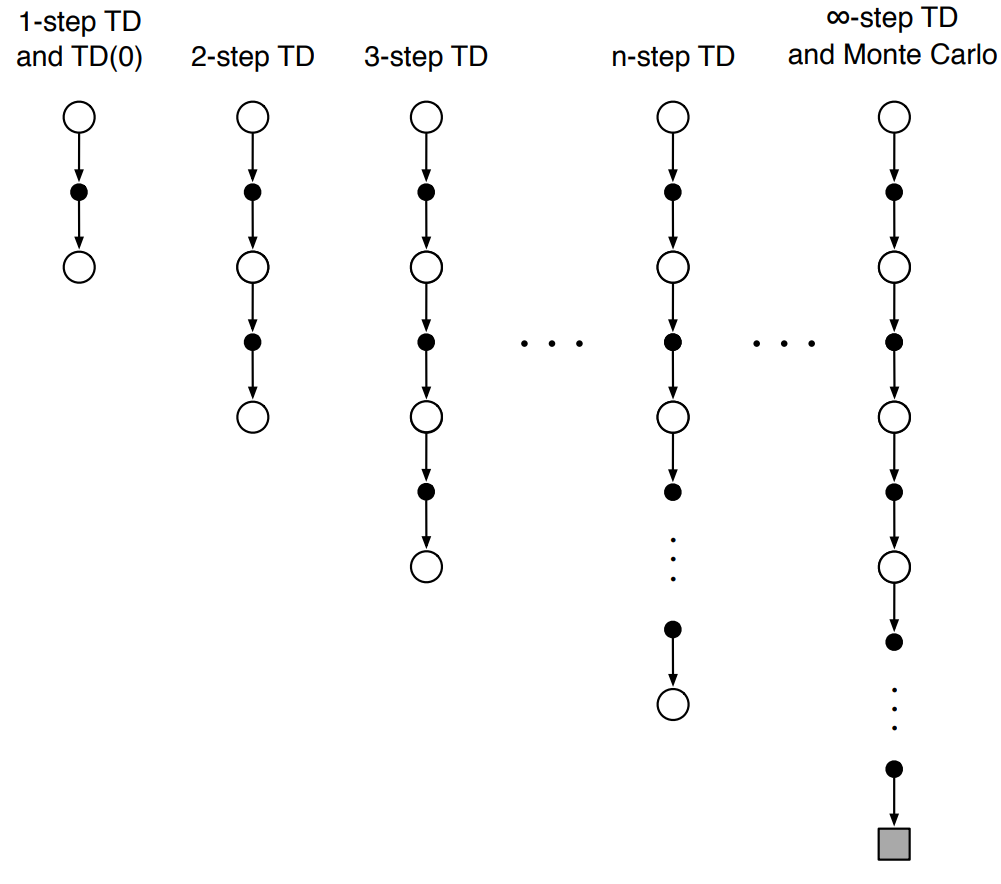
\includegraphics[width=\linewidth]{images/nstep_backup.png}
\end{center}

\begin{center}
    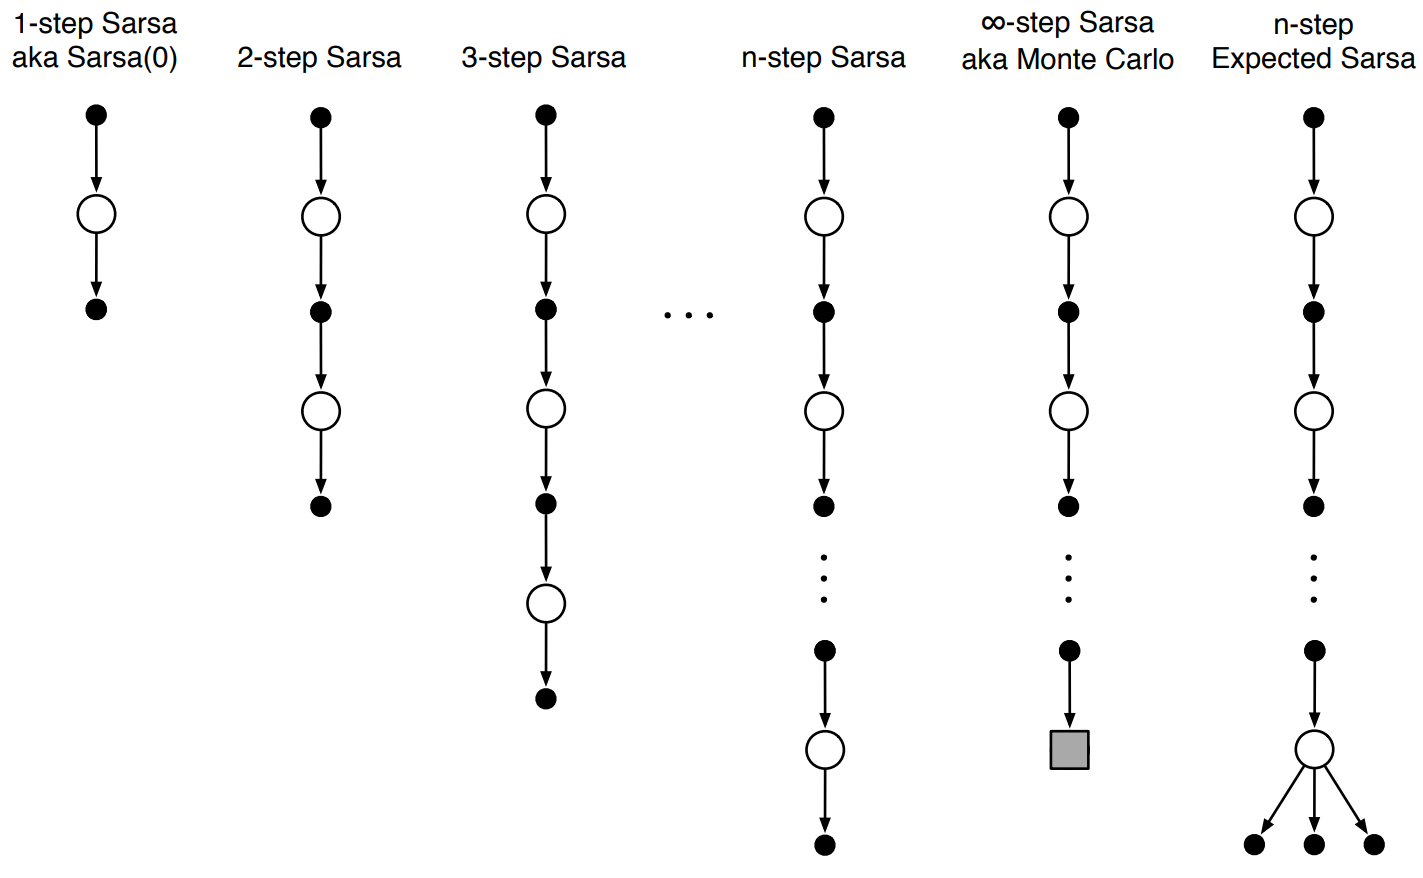
\includegraphics[width=\linewidth]{images/nstep_sarsa_backup.png}
\end{center}
% \end{multicols}

% \newpage

% \begin{multicols}{3}
\section{Planning and Learning}
Planning methods use simulated experience generated by a model, learning methods use real experience generated by the environment. 
Many ideas and algorithms can be transferred between planning and learning.

\begin{algorithm}[H]
 Params: step size $\alpha \in [0,1]$, $\epsilon > 0$\\
 Initialize $Q(s,a)$ for all $s \in \mathcal{S}^+$ and $a in \mathcal{A}(s)$, arbitrarily except that $Q(terminal-state, \cdot) = 0$\\
\ForEach{episode}
{
	1. Select a state $S \in \mathcal{S}$, and an action, $A \in \mathcal{A}(s)$, at random\\
	2. From a Sample Model obtain the sample reward and next state following: R, S' = model (S,A)\\
	3. Apply one-step tabular Q-Learning to $S, A, R, S'$:\\
	$Q(S, A) \leftarrow Q(S, A) + \alpha \left[R + \gamma \max_a Q(S', a) - Q(S, A)  \right]$\\
 }
\caption{Random-sample one-step tabular Q-planning [§8.1]}
\end{algorithm}

\subsection{Dyna}
Within a planning agent, there are at least two roles for real experience: \\
(1) it can be used to improve the model (to match more accurately the real environment), \emph{model learning},\\ 
(2) it can be used to directly improve the value function and policy using the kinds reinforcement learning methods discussed before, \emph{direct RL} [§8.2].\\
\begin{center}
\includegraphics[width=0.6\linewidth]{./images/Planning-Learning.png}
\end{center}
The experience can improve value functions and policies either directly or indirectly via the model (\emph{indirect RL}).
The real experience obtained with the interaction with the environment can be used to improve directly the Policy/value function (direct RL) or indirectly through the model learning and the planning that use simulated experience (\emph{indirect RL}) [§8.2].\\
\begin{center}
\includegraphics[width=0.8\linewidth]{./images/Dyna.png}
\end{center}

\begin{algorithm}[H]
 Initialize $Q(s,a)$ and $Model(S,A)$ for all $s \in \mathcal{S}^+$ and $a \in \mathcal{A}(s)$\\
\While{forever}
{
	(a) $S \leftarrow$ current (nonterminal) state \\
	(b) $A \leftarrow \epsilon$-greedy$(S, Q)$ \\
	(c) Take action $A$; observe resultant reward, $R$, and state, $S'$ \\
	(d) $Q(S, A) \leftarrow Q(S, A) + \alpha \left[R + \gamma \max_a Q(S', a) - Q(S, A)  \right]$ \\
	(e) $Model(S, A) \leftarrow R, S'$ (assuming deterministic environment) \\
	(f) \ForEach{n times}
	{
		$S \leftarrow$ random previously observed state \\
		$A \leftarrow$ random action previosuly taken in $S$\\
		$R, S' \leftarrow Model(S, A)$ \\
		$Q(S, A) \leftarrow Q(S, A) + \alpha \left[R + \gamma \max_a Q(S', a) - Q(S, A)  \right]$ \\
	}
 }
\caption{Dyna-Q [§8.2]}
\end{algorithm}

(d) Direct reinforcement learning\\
(e) Model-learning\\
(f) Planning\\

% \vfill\null
% \columnbreak

If (e) and (f) were omitted, the remaining algorithm would be one-step tabular Q-learning.\\

The agent responds instantly to the latest sensory information and yet always planning in the background. Also the model-learning process is in background. As new information is gained, the model is updated to better match reality. As the model changes, the ongoing planning process will gradually compute a different way of behaving to match the new model.\\

Models may be incorrect for many reasons: environment is stochastic and only a limited number of samples have been observed, the model was learned using function approximation that has generalized imperfectly, the environment has changed and its new behaviour has not yet been observed. 
When the model is incorrect, the planning process is likely to compute a suboptimal policy. In some cases, the suboptimal policy computed by planning quickly leads to the discovery and correction of the modeling error. This happens when the model is optimistic, predicting greater reward or better state transition than are actually possible. It is more difficult to correct a model when the environment becomes better than it was before.


% \end{multicols}

% \newpage

% \begin{multicols}{3}

\section{On-policy Prediction with Function Approximation}
We can approximate value function not as a table but as a parametrized functional form: $\hat{v}(s,\mathbf{w}) \sim v_{\pi}(s)$ where $\mathbf{w} \in \mathbb{R}^d$ and the number of weights is much less than the number of states ($d << |\mathcal{S}|$).
The value estimation can be framed as a Supervised Learning problem.\\
The Monte Carlo methods estimate the value function using samples of the return so the input is the state and the targets are the returns (pairs $(S_i, G_i)$). \\
For TD methods the targets are the one-step bootstrap return (pairs $(S_i, R_{i+1} + \gamma \hat{v}(S_{i+1}, \mathbf{w})$).\\
In RL setting, the data is temporally correlated and the full dataset is not fixed and available from the beginning. Moreover, due to the bootstrapping methods (TD, DP), the target labels change.\\
In tabular case the learned values at each state were decoupled -  an update at one state affected no other.
Now making one state's estimate more accurate means making others' less accurate.

\begin{equation}
    \overline{VE}(\mathbf{w})  \stackrel{.}{=} \sum_{s \in \mathcal{S})} \mu(s) \left [ v_{\pi}(s) - \hat{v}(s, \mathbf{w}) \right ]^2 \label{eq:value_error} \numberthis \quad [9.1]  
\end{equation}
where $\mu(s)$ is a state distribution ($\mu(s) \ge 0$ and $\sum_s \mu(s) = 1$) representing how much we care about the error in each state $s$.
Usually to minimize the \ref{eq:value_error} it is used the Stochastic Gradient Descent (SGD):

\begin{align*}
    \mathbf{w}_{t+1} & \stackrel{.}{=} \mathbf{w}_{t} - \frac{1}{2} \alpha \nabla \left [ v_{\pi}(S_t) - \hat{v}(S_t, \mathbf{w}_t) \right ]^2 \numberthis \quad [9.4]\\
& = \mathbf{w}_{t} - \alpha \left [ v_{\pi}(S_t) - \hat{v}(S_t, \mathbf{w}_t) \right ] \nabla \hat{v}(S_t, \mathbf{w}_t) \numberthis \quad [9.5]
\end{align*}
Usually we have only an approximation $U_t$ of $v_{\pi}(S_t)$ but, if $U_t$ is an unbiased estimation of $v_{\pi}(S_t)$, that is $\mathbb{E}[U_t|S_t=s] = v_{\pi}(S_t)$, for each $t$, then $\mathbf{w}_t$ is guaranteed to converge to a local optimum (under the stochastic approximation condition for decreasing $\alpha$). \\
For MC, $U_t \stackrel{.}{=} G_t$ and hence $U_t$ is an unbiased estimation of $v_{\pi}(S_t)$.

\begin{algorithm}[H]
Inputs: $\pi$ - the policy to be evaluated \\
		a differentiable function $\hat{v} : \mathcal{S} \times \mathbb{R}^d \rightarrow \mathbb{R}$ \\
Parameters: step size $\alpha > 0$ \\
Initialize: $\mathbf{w} \in \mathbb{R}^d$ arbitrarily (e.g. $\mathbb{w} = 0$) \\
\While{forever - for each episode}
{
    Generate an episode following $\pi$: $S_0, A_0, R_1, S_1, A_1,..., S_{T-1}, A_{T-1}, R_T$\\
    \ForEach{step of episode, $t=0,1,..., T-1$}
    {
		$\mathbf{w} \leftarrow \mathbf{w} - \alpha \left [ G_t - \hat{v}(S_t, \mathbf{w}_t) \right ] \nabla \hat{v}(S_t, \mathbf{w})$
    }
 }
\caption{Gradient MC - Estimating $v \sim v_{\pi}$ [§9.3]}
\end{algorithm}

% \rule{0.3\linewidth}{0.25pt} \\
% \scriptsize
% \href{https://github.com/linker81/Reinforcement-Learning-CheatSheet}{https://github.com/linker81/Reinforcement-Learning-CheatSheet}

\section{Policy Gradients}
\textbf{Softmax Policy} $$\pi(a|s, \theta) = \frac{e^{h(s,a,\theta)}}{\sum_{b \in \mathcal{A}}e^{h(s,b,\theta)}}$$ where $h(s,a,\theta) = \theta^\top x(s,a)$

\textbf{Gaussian Policy} $$\pi(a|s, \theta) \sim \mathcal{N}(\mu(s, \theta), \sigma^2)$$ where $\my(s, \theta) = \theta^\top x(s)$

\textbf{Policy Optimisation Problem} Given $\pi(a|s, \theta)$ and interaction with MDP $m$, find the optimal choice of $\theta$

\textbf{Policy Gradient Theorem} For any differentiable policy $\pi$, the policy gradient is $$\nabla J(\theta) = \sum_s d_\pi (s) \sum_a q_\pi (s,a) \nabla \pi(a|s, \theta)$$ where $d_\pi(s)$ is the on-policy distribution under $\pi$. \\

\textbf{Episodic Tasks}: start-state value $d_\pi (s) = \sum_{t=0}^\infty \gamma^t Pr\{S_t = s | s_0, \pi\}$
\textbf{Continuous Tasks}: average reward $d_\pi (s) = \lim_{t \rightarrow \infty} Pr\{S_t = s | \pi\}$

$\nabla J(\theta) = \mathbb{E}_\pi [q_\pi(S_t, A_t) \frac{\nabla \pi(A_t | S_t, \theta)}{\pi (A_t | S_t, \theta)} = \mathbb{E}_\pi [q_\pi(S_t, A_t) \ln \nabla \pi(A_t | S_t, \theta)$

\textbf{Without Baseline} $\theta_{t+1} = \theta_t + \alpha(q_\pi(S_t, A_t) \nabla \ln \pi(A_t | S_t, \theta_t))$ \\
\textbf{With Baseline} $\theta_{t+1} = \theta_t + \alpha[(q_\pi(S_t, A_t) - b(S_t)) \nabla \ln \pi(A_t | S_t, \theta_t)]$ where, typically $b(S_t) = \hat{v}(S_t)$

\textbf{REINFORCE} $q_\pi(S_t, A_t) = \mathbb{E}_\pi [G_t | S_t, A_t]$ \\

\textbf{Actor-Critic Methods} $q_\pi(S_t, A_t) \approx R_{t+1} + \gamma \hat{v}(S_{t+1}, w) - (S_{t}, w)$


$$\nabla \ln \pi(A_t | S_t, \theta_t) = \begin{cases}& x(s,a) - \sum_{a'} \pi(a' | s, \theta) x(s, a') \text{ if softmax policy } \\ & (a - \mu(s, \theta)) x(s)/\sigma^2 \text{ if Gaussian policy }\end{cases}$$

\begin{center}
\includegraphics[angle=90,width=1\linewidth]{./images/Tabular_Value_Function.png}
\end{center}
\end{multicols}

\end{document}
